\section{Method}
\label{sec:method}

\begin{figure*}[!t]
\centering
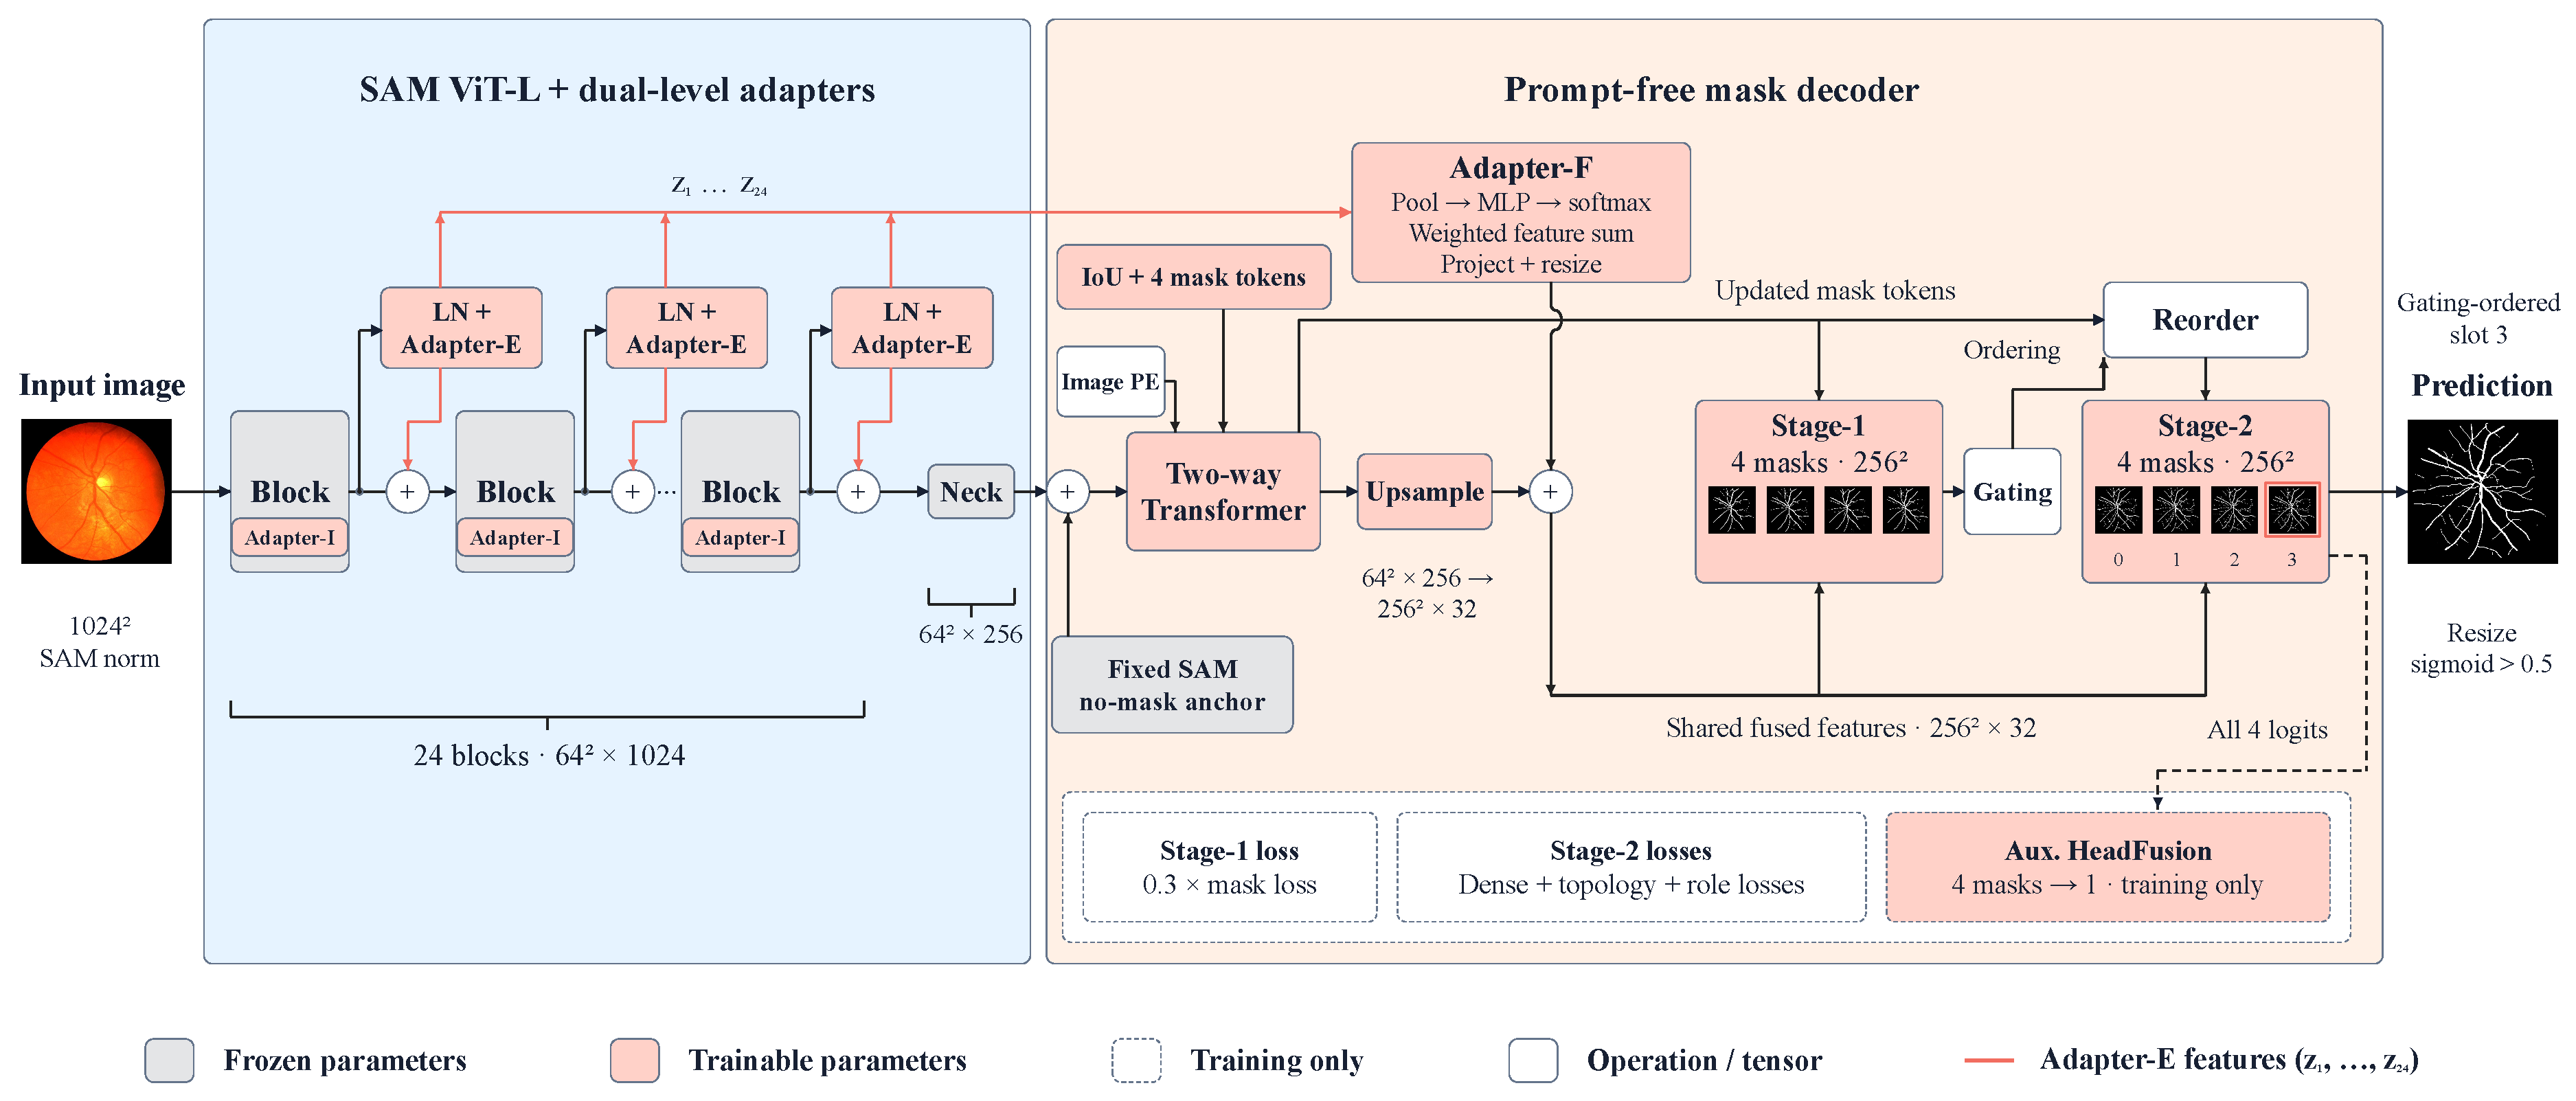
\includegraphics[width=\textwidth]{../img/fig_framework.pdf}
\caption{Overview of DCD.  A frozen SAM ViT-L encoder is adapted with
block-internal Adapter-I and block-external Adapter-E features, which
Adapter-F fuses into the decoder.  Stage-1 ranks four candidate masks by
gating confidence, and Stage-2 refines them with dense, topology, and
role-specific losses.  At inference, DCD deploys a fixed slot (slot~3),
without a test-time selector or the training-only fusion branch.}
\label{fig:dcd_framework}
\end{figure*}

\subsection{Overview}
\label{sec:method_overview}

DCD studies deployment of a prompt-free multi-candidate decoder. Given 18
support images from six datasets, it predicts one binary mask without points
or target-domain support. It is evaluated on unseen datasets with the same
structure classes but different sources or modalities, and on novel classes
absent from training.

The starting point is SACM's prompt-free pipeline~\cite{zhu2026sacm}. Its SAM
ViT-L encoder remains frozen and is adapted by two bottleneck residual MLPs:
Adapter-I inside each Transformer block and Adapter-E at each block boundary.
For the $l$-th block,
\begin{equation}
a_l^{I}(u)=W_l^{\mathrm{up}}\,\sigma\!\left(W_l^{\mathrm{down}}\,\mathrm{LN}(u)\right),
\label{eq:adapter_i}
\end{equation}
\begin{equation}
x_{l+1}=x_l+a_l^{E}(\mathrm{LN}(x_l)),
\label{eq:adapter_e}
\end{equation}
where $\sigma$ is GELU. Adapter-I adds its output to the MLP residual, while
Adapter-E updates the block output and passes context to the next block.
Adapter-F gives the decoder a cross-layer view by pooling each Adapter-E
output into a descriptor $z_l$, weighting the 24 descriptors with softmax, and
adding the weighted sum to the upsampled decoder feature:
\begin{equation}
\alpha=\mathrm{softmax}\!\left(\mathrm{FFN}([z_1;\dots;z_{24}])\right),
\label{eq:fusion_weights}
\end{equation}
\begin{equation}
F\leftarrow F+\mathrm{MLP}_F\!\left(\sum_{l=1}^{24}\alpha_l e_l\right).
\label{eq:fusion}
\end{equation}
The prompt encoder is frozen, and the dense prompt is a learned no-mask
embedding; only the adapters, fusion MLP, and decoder are trained. The decoder
exposes four candidate heads, which gives complementary hypotheses but creates
an inference-time choice.

\subsection{Candidate Generation and Ranking}
\label{sec:method_candidates}

The decoder contains one IoU token and four mask tokens. A Two-way Transformer
updates these tokens with the image feature and the dense prompt, and four
Stage-1 MLPs produce coarse masks. For each candidate, the maximum spatial
activation serves as a gating score; the scores order the candidates before
Stage-2 refinement:
\begin{equation}
M_k^{(1)}=\mathrm{MLP}_k^{(1)}(t_k;F),\qquad
g_k=\max_{u}M_k^{(1)}(u),
\label{eq:stage1}
\end{equation}
\begin{equation}
s=\mathrm{argsort}\!\left(\mathrm{softmax}(g)\right),\qquad
M_j^{(2)}=\mathrm{MLP}_j^{(2)}(t_{s_j};F),
\label{eq:stage2}
\end{equation}
where $k,j=0,\dots,3$, $t_k$ is the $k$-th mask-token descriptor, and $F$ is
the decoder feature. Slot~0 is the gating champion, and slot~3 is the
last-ranked candidate on every image. The IoU prediction head is neither
supervised nor used at inference.

This ranking is not a selector: it defines a training anchor and a stable
order, while inference replaces it with a fixed slot. Keeping the same
candidate experts in both stages isolates deployment from training.

\subsection{Role-Specialized Supervision}
\label{sec:method_supervision}

All Stage-2 heads share the decoder feature but have separate output MLPs and
different objectives, so they can specialize. The champion anchors the dense
and topology terms with full weight, while the three auxiliary heads share a
total weight of 0.25. Every Stage-2 head receives a dense BCE+Dice loss and,
after a short warmup, is regularized by soft-clDice~\cite{shit2021cldice} and
Skeleton Recall~\cite{kirchhoff2024skeletonrecall}. The dense term weights BCE
and Dice as $0.7$ and $0.3$, with a foreground weight of 2 for BCE. The
topology term adds 0.1 soft-clDice and 0.1 Skeleton Recall per head and is
ramped from 0 to 1 between epochs 5 and 10. Every Stage-1 head is also
deep-supervised with the dense loss.

The three auxiliary slots receive role losses with total weight 0.1. Slot~1
is pushed toward topology by an extra soft-clDice term. Slot~2 targets
boundaries with a BCE+Dice loss whose pixels are weighted by $1+4B$ on a
$5\times5$ boundary band $B$. Slot~3 targets recall with a Tversky loss using
$\alpha=0.3$ and $\beta=0.7$, where
$\ell_{\mathrm{tv}}=1-TP/(TP+0.3FP+0.7FN)$ and $TP$, $FP$, and $FN$ are pixel
counts. A zero-initialized $1\times1$ convolution fuses the four refined masks
into an auxiliary output, which equals the champion at initialization and is
discarded after training.

With $\ell_1=\ell_{\mathrm{clDice}}(M_1^{(2)},y)$,
$\ell_2=\ell_{\mathrm{bnd}}(M_2^{(2)},y)$, and
$\ell_3=\ell_{\mathrm{tv}}(M_3^{(2)},y)$, the role and total objectives are
\begin{equation}
\mathcal{L}_{\mathrm{role}}=0.1\left(\ell_1+\ell_2+\ell_3\right),
\label{eq:role}
\end{equation}
\begin{equation}
\mathcal{L}=\mathcal{L}_{\mathrm{dense}}+\mathcal{L}_{\mathrm{top}}
+\mathcal{L}_{\mathrm{role}}+\ell_{\mathrm{fus}}+0.3\,\mathcal{L}_{\mathrm{ds}},
\label{eq:total}
\end{equation}
where $\ell_{\mathrm{fus}}=\ell_{\mathrm{dense}}(M_{\mathrm{fus}},y)$,
$\ell_{\mathrm{bnd}}=\mathrm{BCE}_{1+4B}+1-\mathrm{Dice}$,
$\mathcal{L}_{\mathrm{dense}}$ and $\mathcal{L}_{\mathrm{top}}$ are the
weighted dense and topology terms over all Stage-2 heads, and
$\mathcal{L}_{\mathrm{ds}}$ is the averaged deep supervision of the four
Stage-1 heads. Exact resolutions and the warmup schedule are listed in the
supplement.

\subsection{Deterministic Deployment}
\label{sec:method_deploy}

Training uses gating to order the candidates and to anchor the losses. For
deployment we derive an inference-only checkpoint in which the selection rule
is fixed and the fusion branch is removed; the candidate and adapter weights
are unchanged, so no retraining is required. The checkpoint sets
\texttt{head\_select=fixed}, \texttt{deployment\_head=3}, and
\texttt{head\_fusion=0}, and drops the fusion tensors. Gating still computes
the order, but DCD returns the Stage-2 mask in slot~3, thresholded at 0.5 and
resized to the ground-truth resolution. The fused output and the IoU predictor
are not used. The slot is selected on the validation split and then frozen for
all test datasets and seeds.

Fixing the slot is motivated by two observations. Slot~3 is the
recall-oriented Tversky expert, so fixing its rank preserves specialization
and removes per-image selector variance. A jointly trained selector can also
co-adapt with the heads and drift under a change in modality or acquisition
conditions. Fixed deployment removes this decision point, while the candidate
experts themselves are unchanged. Training uses the hyperparameters listed in
the supplement.
